%% ---------------------------------------------------------------------------------------------------------------------

\chapter{\textit{go-geiger}: Identification of Unsafe Usage}\label{ch:go-geiger}

This chapter presents \toolGeiger{}, a tool to find usages of the \unsafe{} \acrshort{API} in Go packages and their
dependencies.
Furthermore, an empirical study on \unsafe{} usage in open-source projects using \toolGeiger{} is shown, and a novel
data set of labeled samples of \unsafe{} code is described.
Figure~\ref{fig:outline4} shows which parts of the contributions of this thesis are given in this chapter.

\begin{figure}[htp!]
    \includegraphics[width=\textwidth]{assets/figures/chapter4/outline4.pdf}
    \caption{Organization of Chapter 4}
    \label{fig:outline4}
\end{figure}



%% ---------------------------------------------------------------------------------------------------------------------

\section{Design}\label{sec:go-geiger:design}

The novel tool \toolGeiger{} is designed to identify usages of the \unsafe{} \acrshort{API} in Go source code.
In contrast to existing tools like \toolGosec{}, it includes the dependencies of Go packages in the analysis, which
gives a much better picture of possible \unsafe{} usages.
It is inspired by \toolCargoGeiger{}\footnote{\url{https://github.com/rust-secure-code/cargo-geiger}}, a similar tool
for detecting the use of unsafe code blocks in Rust programs.
Figure~\ref{fig:go-geiger-architecture} shows the architecture of \toolGeiger{}.

\begin{figure*}[t!]
    \includegraphics[width=\textwidth]{gfx/figures/go-geiger-architecture.png}
    \caption{Go-Geiger Unsafe Detection Tool Design}
    \label{fig:geiger-architecture}
\end{figure*}


First, the dependency tree of the packages that are given for analysis is built.
Then, the sources of all the packages in this tree are parsed, and the resulting abstract syntax tree (\acrshort{AST})
is inspected.
Within the \acrshort{AST}, usages of the \unsafe{} \acrshort{API} are identified.
Each usage is assigned a tuple of labels consisting of \textit{match type} and \textit{context type}.
The match type represents the part of the \unsafe{} \acrshort{API} that is used.
It can be either of the four \unsafe{} package members \textit{Pointer}, \textit{Sizeof}, \textit{Offsetof}, and
\textit{Alignof}, the \textit{reflect} package fields \textit{SliceHeader} and \textit{StringHeader}, or the
\textit{uintptr} keyword.
The context type indicates the functional part of code that the usage is found in.
It can be either an \textit{assignment}, a \textit{call} of a function, a function \textit{parameter} definition, or a
\textit{variable} definition.
If the context can not be assigned to one of these four options, then it is set to \textit{other}.
This context allows to filter the search for \unsafe{} usages to particular functional code positions.
There is a \toolGeiger{} command line parameter to request this filtering.
For example, it is possible to count only \unsafe{} usages that are used within parameters of function calls.
After the \unsafe{} usages are identified, they are counted.
For this, it is necessary to take care of package deduplication.
If a particular package exists in the dependency tree multiple times and is reachable on different paths, it must still
be counted only once when calculating the sum of \unsafe{} usages in a package's dependencies.
This is because the package does not get any less safe by including the same code multiple times, the code is already
part of the resulting program.
Finally, the analysis results are shown to the user.
It is possible to output the \unsafe{} usage counts as well as the lines of code containing the usages.

The source code and documentation of \toolGeiger{} is available on
\github{}\footnote{\url{https://github.com/jlauinger/go-geiger}}.
It can be installed using the standard Go \acrshort{CLI} tool.
To execute it, append the package names that should be checked as parameters.
For example, to examine a local package for \unsafe{} usages run \textit{go-geiger ./my/package}.
There is no limitation on the number of packages that can be supplied as parameters.
Figure~\ref{fig:go-geiger-screenshot} shows a screenshot of \toolGeiger{}.
It presents the analyis results for the \textit{go-geiger} source code itself.
The output is truncated is missing parts of the table with \unsafe{} counts, which have been excluded to decrease the
space needed to display the figure.

\begin{figure}[htp!]
    %\vspace{2mm}
    \centering
    \includegraphics[width=\textwidth]{assets/images/chapter4/go-geiger-screenshot.png}
    \caption{Usage example screenshot of \toolGeiger{}}
    \label{fig:go-geiger-screenshot}
    %\vspace{-14pt}
\end{figure}


The output shown in Figure~\ref{fig:go-geiger-screenshot} is composed of three parts.
The first is a table showing the \unsafe{} usage counts for each package in the dependency tree for the packages
given for analysis.
The first column indicates the total number of usages in the package including all its dependencies.
The second column shows the number for the package alone, without the dependencies.
The heading for this column is \textit{local package}.
Next, there are five columns with individual usage counts for the four possible usage contexts described above,
\textit{variable}, \textit{parameter}, \textit{assignment}, \textit{call}, as well as \textit{other} for all matches
that could not be assigned to any of them.
These columns add up to the \textit{local package} count.
Finally, the import path for the package is given to identify it.
Lines that are printed in green (the last \checkNum{two} lines in Figure~\ref{fig:go-geiger-screenshot}) represent
packages with no local \unsafe{} usages.
Red lines (e.g. the \checkNum{seventh} line) are packages that directly contain \unsafe{} code, and white lines indicate
that the package does not contain \unsafe{} usages itself but instead introduces them through its dependencies.
After the table, there is a summary of the number of packages belonging into these three categories green, red, and
white, and finally a legend for the colors.


%% ---------------------------------------------------------------------------------------------------------------------

\section{Implementation}\label{sec:go-geiger:implementation}

The identification of the dependency tree for the packages to analyze, as well as the parsing of the source code is done
using the standard Go compiler toolchain.
It is accessable using the \textit{packages}
\acrshort{API}\footnote{\url{https://pkg.go.dev/golang.org/x/tools/go/packages}}.
Similarly, the inspection of the \acrshort{AST} is done using the \acrshort{API} available though the \textit{ast}
package in Go\footnote{\url{https://golang.org/pkg/go/ast/}}.

To find \unsafe{} usages corresponding to the different match types shown in Figure~\ref{fig:go-geiger-architecture},
the \acrshort{AST} is filtered for \textit{SelectorExpr} and \textit{Ident} nodes.
The first represent selector expressions, which indicate possible access of a member of another package, like in a usage
of \textit{unsafe.Pointer}.
The second is used to find instances of \textit{uintptr}.
In both cases the concrete identifier names in the \acrshort{AST} nodes are checked to distinguish \unsafe{} usages from
arbitrary other field accesses.
The context type is determined by going up in the \acrshort{AST} starting at the expression node corresponding to a
given \unsafe{} usage.
For example, an \unsafe{} usage is considered part of the \textit{assignment} context type if it is a descendent of
either an \textit{AssignStmt}, \textit{CompositeLit}, or \textit{ReturnStmt} node.
The \textit{call}, \textit{parameter}, and \textit{variable} classes correspond to \textit{CallExpr}, \textit{FuncDecl},
and \textit{GenDecl} nodes, respectively.
To achieve an effective assignment of the context type, the order in which the different types are checked is important.
This is because an \unsafe{} usage have reason to be included in several context types such as \textit{call} and
\textit{assignment} in an example like \textit{x := f(unsafe.Pointer(y))}.

The \unsafe{} usage counts are first collected for each package.
A cache is used to avoid analyzing the same package multiple times if it is present several times in the dependency
tree.
When the usage count including dependencies is calculated, \toolGeiger{} starts with the root packages that were
requested for analysis by the user, and recursively calculates the respective counts.
Again, the cache is used to avoid summing up multiple times.
This approach is a depth-first traversal of the dependency tree.

Automated acceptance testing verifies that \toolGeiger{} works as intended.
The test is done by running \toolGeiger{} on a test fixture package with a known number of \unsafe{} usages.
Then, the output is checked for the expected usage counts.


%% ---------------------------------------------------------------------------------------------------------------------

\section{Evaluation}\label{sec:go-geiger-evaluation}

A major contribution of this thesis is an analysis of unsafe code usage in the wild:
the top 500 most popular open source Go projects.

Threat to validity: unable to differentiate dead code in analysis.
This is similar to many studies as summarized in the related work chapter.


%% ---------------------------------------------------------------------------------------------------------------------

\subsection{Data Set}\label{subsec:go-geiger:evaluation:data-set}

Description of how the data set was generated and processed


%% ---------------------------------------------------------------------------------------------------------------------

\subsection{Usages in Projects and Dependencies}\label{subsec:go-geiger:evaluation:unsafe-usage}

Including import depth analysis

\begin{figure}[!t]
    \vspace{-12pt}
    \centering
    \includegraphics[width=0.43\textwidth]{gfx/figures/distribution-unsafe-types-pdf.pdf}
    \caption{Distribution of different types of \unsafe{} tokens}
    \label{fig:unsafe-tokens-distribution}
\end{figure}
\begin{figure*}[!t]
    \centering
    \includegraphics[width=\textwidth]{gfx/figures/unsafe-import-depth.png}
    \caption{Import Depth of Unsafe Packages. Answers~\ref{rq:depsDepth}: unsafe packages are around \averageUnsafeImportDepth{} hops away (sd=\stdUnsafeImportDepth), thus manageable to find manually.}
    \label{fig:unsafe-import-depth}
\end{figure*}

\begin{figure}[!t]
    %\vspace{2mm}
    \centering
    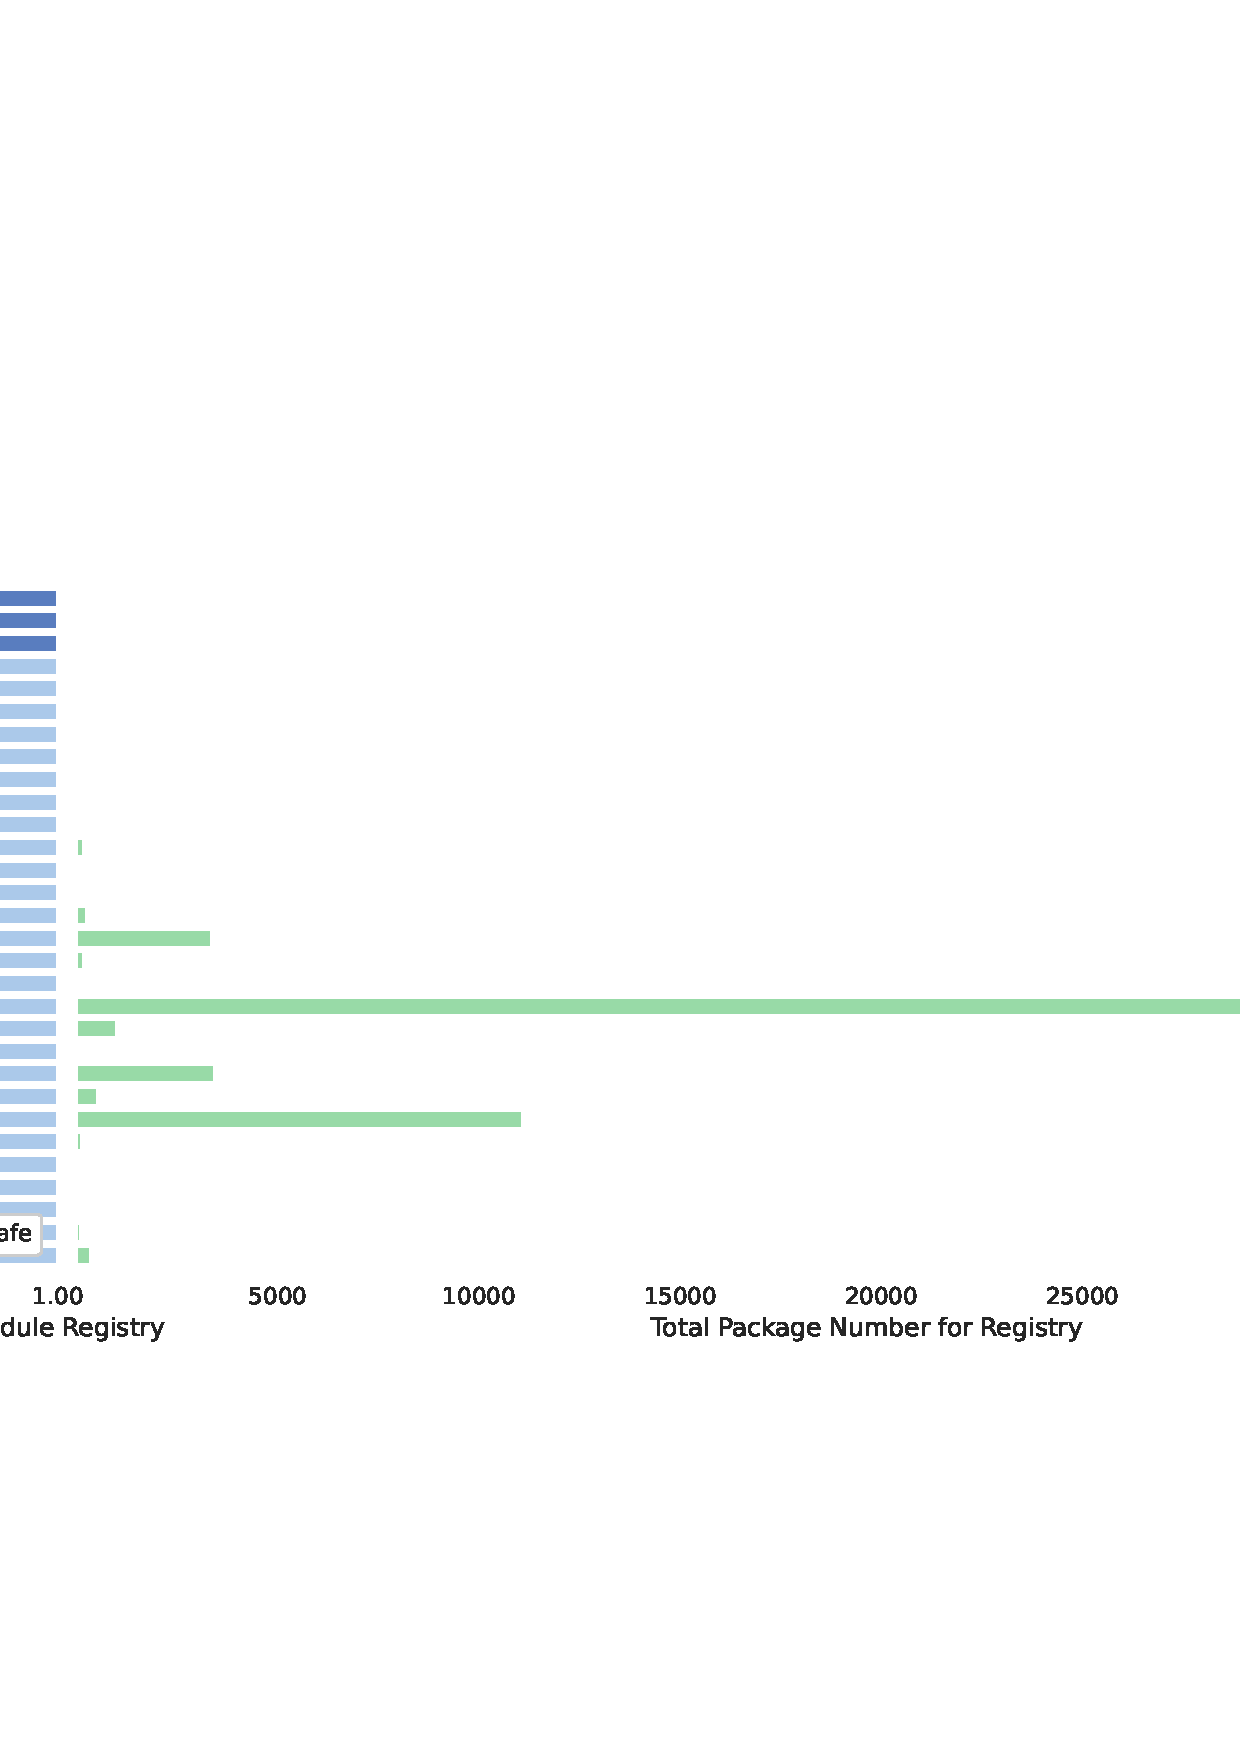
\includegraphics[width=\textwidth]{assets/plots/chapter4/unsafe-packages-by-registry-n30.pdf}
    \caption{Share and Total Number of Unsafe Packages by Registries for the 30 Registries with Most Unsafe Packags}
    \label{fig:unsafe-packages-by-registry-n30}
    %\vspace{-10pt}
\end{figure}



%% ---------------------------------------------------------------------------------------------------------------------

\subsection{Influence of Popularity}\label{subsec:go-geiger:evaluation:popularity}

Correlation with Project Star / Forks Stats, Age, etc.

\todo{Add scatter plot that shows correlation between unsafe usage and project stars/forks/age using differently colored
dots. It should result in no correlation.}


%% ---------------------------------------------------------------------------------------------------------------------

\subsection{Change of Usage over Time}\label{subsec:go-geiger:evaluation:over-time}

\begin{table}[htp!]
    \centering
    \caption{Change of unsafe usage over time in the golang.org/x/sys module}
    \label{tbl:unsafe-usage-over-time}
    \begin{tabular}{l|l|r}
    \textbf{Version}                   & \textbf{Release date} & \textbf{Unsafe usage count} \\
    \hline
    v0.0.0-20171012164349-43eea11bc926 & 12.10.2017            & 315                         \\
    v0.0.0-20190502145724-3ef323f4f1fd & 02.05.2019            & 387                         \\
    v0.0.0-20190726091711-fc99dfbffb4e & 26.07.2019            & 392                         \\
    v0.0.0-20191001151750-bb3f8db39f24 & 01.10.2019            & 403                         \\
    v0.0.0-20191128015809-6d18c012aee9 & 28.11.2019            & 403                         \\
    v0.0.0-20200107162124-548cf772de50 & 07.01.2020            & 428                         \\
    v0.0.0-20200302150141-5c8b2ff67527 & 02.03.2020            & 428                         \\
    v0.0.0-20200413165638-669c56c373c4 & 13.04.2020            & 434                         \\
    v0.0.0-20200501145240-bc7a7d42d5c3 & 01.05.2020            & 440                         \\
    \end{tabular}
\end{table}


%% ---------------------------------------------------------------------------------------------------------------------

\subsection{Comparison with Existing Tools}\label{subsec:go-geiger:evaluation:linters-comparison}

\toolVet{}, \toolGosec{}

\input{assets/tables/chapter4/go-geiger-linter-comparison.tex}


%% ---------------------------------------------------------------------------------------------------------------------

\section{Purpose of Unsafe in Practice: a Labeled Data Set}\label{sec:go-geiger:labeled-dataset}

This chapter contributes an in-depth study of unsafe usages in 10 selected open-source Go projects.
I analyzed 1000 usages in application code, and 400 usages in the standard library.
The usages are classified in two dimensions by what is happening and what is the higher-level purpose.

I analyzed the following projects.

\begin{table}[htp!]
    \centering
    \caption{Projects selected for labeled data set}
    \label{tbl:dataset-projects}
    \begin{tabular}{llrrl}
        {} & \textbf{Name} &  \textbf{Stars} &  \textbf{Forks} &    \textbf{Revision} \\ \hline
        \rowcolor{verylightgray}
        1  &         kubernetes/kubernetes &  66,512 &  23,806 &  \texttt{fb9e1946b0} \\
        2  &                 elastic/beats &   8,852 &   3,207 &  \texttt{df6f2169c5} \\
        \rowcolor{verylightgray}
        3  &             gorgonia/gorgonia &   3,373 &    301 &  \texttt{5fb5944d4a} \\
        4  &              weaveworks/scope &   4,354 &    554 &  \texttt{bf90d56f0c} \\
        \rowcolor{verylightgray}
        5  &  mattermost/mattermost-server &  18,277 &   4,157 &  \texttt{e83cc7357c} \\
        6  &               rancher/rancher &  14,344 &   1,758 &  \texttt{56a464049e} \\
        \rowcolor{verylightgray}
        7  &                 cilium/cilium &   5,501 &    626 &  \texttt{9b0ae85b5f} \\
        8  &                     rook/rook &   7,208 &   1,472 &  \texttt{ff90fa7098} \\
        \rowcolor{verylightgray}
        9  &             containers/libpod &   4,549 &    539 &  \texttt{e8818ced80} \\
        10 &                       xo/usql &   5,871 &    195 &  \texttt{bdff722f7b} \\
    \end{tabular}
\end{table}

I selected them based on their high number of unsafe usages, and taking care of that they represent a reasonably large
diversity.
The projects contain applications based around containers and operations, chat, infrastructure as a service, data
storage, visualization, and machine learning.

When selecting samples to look at, I deliberately separated the standard library from application usages.
This is based on the results of the large-scale study shown in Chapter~\ref{ch:survey}, which show that all projects
must use the standard library, and the hypothesis that the standard library uses unsafe patterns differently.
It has to do so because the standard library takes care of low-level memory management by design.

Standard library is defined by the packages that live in the Go standard library and the \texttt{golang.org/x/sys}
module.
I took the decision to include the sys package because it contains a lot of syscall infrastructure and in general
behaves more like the standard library than application code.
It is also maintained by the core Go developer team.
Obviously, application packages is defined as packages that are not part of the standard library.

I randomly sampled 1000 snippets from application packages and 400 snippets from the standard library.
The samples are taken without duplicates in version, that is the same snippet by module, file, and line number is not
taken twice if there is a different version of the same module also available.
This is done by best effort: if the line number changes between module versions there might still be logical
duplication.
The set of deduplication is module, package, file, line number.
I only took samples that contain \texttt{unsafe.Pointer}, no other unsafe matches.

Both because there is no easy way to find out if an imported dependency is maintained by a project itself, or by a
third party, and because it gives a better picture on real unsafe usages in the industry, the unsafe samples are taken
from all dependencies.
Therefore, the snippets are not all part of packages from the ten projects, but some more packages.

I classified the samples on two dimensions.
The first shows what is being done, e.g. a cast or a pointer arithmetic.
The second dimension shows the purpose of the unsafe usage, e.g. serialization or realization of generics.

The results are shown in Table~\ref{tbl:labels-results-app} for the application code snippets, and
Table~\ref{tbl:labels-results-std} for the standard library snippets.

\begin{table*}[!t]
    \centering
    \caption[Labeled unsafe.Pointer usages in application code and standard library samples]%
    {Labeled unsafe.Pointer usages in application code and standard library samples \newline \tiny ~ \newline \small
        \underline{eff}: efficiency, \underline{gen}: generics, \underline{ser}: (de)serialization,
        \underline{inev}: inevitable use, \underline{SR}: safer reflections, \underline{LC}: layout control,
        \underline{EA}: hide from escape analysis, \underline{UU}: unused, \underline{cgo}: CGo mechanics,
        \underline{no GC}: avoid garbage collector, \underline{typ}: types implementation,
        \underline{mem}: memory management \newline \tiny ~}
    \label{tbl:dataset-classes}
    \begin{adjustbox}{max width=\textwidth}
    \begin{tabular}{r|cc|cc|cc|cc|cc|cc|cc|cc|cc|cc|cc|cc|cc}
                          & \multicolumn{2}{c|}{eff} & \multicolumn{2}{c|}{gen} & \multicolumn{2}{c|}{ser} & \multicolumn{2}{c|}{inev} & \multicolumn{2}{c|}{SR} & \multicolumn{2}{c|}{LC} & \multicolumn{2}{c|}{EA} & \multicolumn{2}{c|}{UU} & \multicolumn{2}{c|}{cgo} & \multicolumn{2}{c|}{no GC} & \multicolumn{2}{c|}{typ} & \multicolumn{2}{c|}{mem} & \multicolumn{2}{c}{total} \\ \hline
                          &  app &  std &  app &  std &  app &  std &  app &  std &  app &  std &  app &  std &  app &  std &  app &  std &  app &  std &   app &  std &  app &  std &  app &  std &   app &  std \\ \hline
 conversion-struct-struct &  408 &    4 &   42 &      &    3 &    6 &    1 &      &    1 &      &      &      &      &    2 &      &      &    5 &    2 &       &      &      &   30 &      &    4 &   460 &   48 \\
\rowcolor{verylightgray}
  conversion-struct-basic &   90 &    2 &   27 &      &    2 &    2 &      &    2 &      &      &    2 &    1 &      &      &      &      &    2 &    1 &       &      &      &    1 &      &    7 &   123 &   16 \\
        conversion-header &   37 &    1 &    2 &      &    1 &      &      &      &      &      &      &      &      &      &      &      &      &      &       &      &      &    2 &      &    1 &    40 &    4 \\
\rowcolor{verylightgray}
  conversion-struct-bytes &   26 &    5 &    2 &      &   73 &    6 &      &      &      &      &    2 &    1 &      &      &      &      &    1 &      &       &      &      &    1 &      &      &   104 &   13 \\
       conversion-pointer &   14 &   20 &    8 &      &      &      &    1 &      &    1 &      &      &      &      &      &      &      &   13 &    1 &       &      &      &    9 &      &    3 &    37 &   33 \\
\rowcolor{verylightgray}
     direct-memory-access &    2 &    1 &   10 &      &    1 &      &    1 &      &      &      &    5 &      &      &      &      &      &      &      &       &      &      &    4 &      &    8 &    19 &   13 \\
       pointer-arithmetic &    7 &    4 &    1 &      &      &      &      &      &    1 &      &    7 &    2 &    1 &    2 &      &      &      &    1 &       &      &      &    8 &      &    9 &    17 &   26 \\
\rowcolor{verylightgray}
               definition &    6 &      &    4 &    1 &      &      &      &      &   20 &    1 &    1 &      &      &      &    1 &      &    4 &    4 &       &      &      &    8 &      &   12 &    36 &   26 \\
                 delegate &    3 &      &   58 &    1 &      &      &   33 &   59 &      &      &      &      &      &    5 &      &      &    9 &    1 &       &      &      &    2 &      &    6 &   103 &   74 \\
\rowcolor{verylightgray}
          type-reflection &      &      &   25 &      &      &      &      &      &    3 &      &      &      &      &      &      &      &      &      &       &      &      &    1 &      &      &    28 &    1 \\
                  syscall &      &      &      &      &      &      &      &      &      &      &      &      &      &      &      &      &      &      &    17 &  138 &      &      &      &      &    17 &  138 \\
\rowcolor{verylightgray}
                   unused &      &      &      &      &      &      &      &      &      &      &      &      &      &      &   16 &    8 &      &      &       &      &      &      &      &      &    16 &    8 \\ \hline
                        total &  593 &   37 &  179 &    2 &   80 &   14 &   36 &   61 &   26 &    1 &   17 &    4 &    1 &    9 &   17 &    8 &   34 &   10 &    17 &  138 &    0 &   66 &    0 &   50 &  1000 &  400 \\
\end{tabular}
    \end{adjustbox}
\end{table*}

I put each sample along with its classification and information about where it was taken from into its own file.
The files are put into directories whose names indicate both classification dimensions.

Here are examples and descriptions for each of the classes used to describe what is happening in an unsafe usage.

\begin{lstlisting}[language=Golang, label=lst:dataset-label-class-examples, caption=Example code snippets for different classes in the data set]
// cast-basic, efficiency
out.TimeoutSeconds = (*int32)(unsafe.Pointer(in.TimeoutSeconds))

// cast-bytes, serialization
return (*(*[SizeofTcTbfQopt]byte)(unsafe.Pointer(x)))[:]

// cast-header, efficiency
hdr := &reflect.SliceHeader{
    Data: uintptr(unsafe.Pointer(&data[i])),
    Len:  stride,
    Cap:  stride,
}
retVal = append(retVal, *(*[]uint8)(unsafe.Pointer(hdr)))

// cast-pointer, serialization
func lookupGoTypeUnfolder(to interface{}) (unsafe.Pointer, ptrUnfolder) {
    switch ptr := to.(type) {
    case *interface{}:
        return unsafe.Pointer(ptr), newUnfolderIfc()
    // ...

// cast-struct, efficiency
out.Configuration = (*runtime.Unknown)(unsafe.Pointer(in.Configuration))

// definition, serialization
type unsafeType struct {
    safeType
    rtype    unsafe.Pointer
    ptrRType unsafe.Pointer
}

// delegate, serialization
func (encoder *dynamicEncoder) Encode(ptr unsafe.Pointer, stream *Stream) {
    obj := encoder.valType.UnsafeIndirect(ptr)
    stream.WriteVal(obj)
}

// memory-access, serialization
deReferenced := *((*unsafe.Pointer)(ptr))
if deReferenced == nil {
    return true
}

// pointer-arithmetic, layout
unaligned := brokenUnaligned && uintptr(unsafe.Pointer(&value[0]))&3 != 0

// syscall, no-gc
n, _, errno := syscall.Syscall(syscall.SYS_RECVMSG, s, uintptr(unsafe.Pointer(h)), uintptr(flags))

// unused, unused
func (encoder emptyArrayEncoder) Encode(ptr unsafe.Pointer, stream *Stream) {
    stream.WriteEmptyArray()
}
\end{lstlisting}



%\section{Evaluation}
%
%%% -----------------------------------------------------------------------------
%
%\chapter{Survey of unsafe code usages in popular Go projects}\label{ch:survey}
%
%
%
%%% -----------------------------------------------------------------------------
%
%\section{Most popular open source Go projects}\label{sec:most-popular-projects}
%
%I downloaded the top 500 most popular (by number of stars) Go projects from Github.
%They can be found through Github search.
%
%Using the \texttt{github.com/google/go-github/github}~\cite{gogithub} and \texttt{github.com/go-git/go-git/v5}~\cite{gogit}
%Go libraries, I found, saved, downloaded, and checkout out these projects using a Go program.
%
%The projects, including the revision I checked out, and some meta data is shown in Table~\ref{tbl:projects}.
%
%
%%% -----------------------------------------------------------------------------
%
%\section{Methods of generating data points}\label{sec:survey-acquisition-methods}
%
%Iteration of three data acquisition programs, getting faster and faster: Bash, Python, Go.
%
%Loading packages used by the program by running \texttt{go list -deps -json ./...}, then parsing the JSON output.
%
%CSV is used to write data to disk.
%Interop with Go structure types is achieved using the \texttt{github.com/gocarina/gocsv}~\cite{gocsv} library.
%
%Program uses the following steps:
%
%\begin{enumerate}
%    \item Read projects to analyze from CSV file
%    \item Get package list for a given project
%    \item Run requested analysis type
%    \item Parse output and match findings to package and file
%    \item Append findings for this project to CSV file
%    \item Continue with step 2 for the next project, until done
%\end{enumerate}
%
%There are five different analysis types:
%
%\begin{itemize}
%    \item Grep
%    \item Go Vet
%    \item Gosec
%    \item Abstract Syntax Tree
%    \item My linter (go-safer)
%\end{itemize}
%
%The time needed to run these analysis on the 500 projects described in Section~\ref{sec:most-popular-projects} is shown
%in Table~\ref{tbl:survey-analysis-wallclocktime}.
%
%\begin{table}[h]
%    \centering
%    \caption{Wall-clock runtime for different analysis types used for the data survey}
%    \label{tbl:survey-analysis-wallclocktime}
%    \begin{tabular}{ll}
%        \toprule
%        Analysis Type & Wall-Clock Time \\
%        \midrule
%        (Project Download) & 4 hours \\
%        Grep & 15 minutes \\
%        Go Vet & 3 hours \\
%        Gosec & 24 hours \\
%        Abstract Syntax Tree & 1 hour \\
%        Go-Safer Linter & 3.5 hours \\
%        \bottomrule
%    \end{tabular}
%\end{table}
%
%
%%% -----------------------------------------------------------------------------
%
%\section{Description and structure of data set}\label{sec:survey-dataset}
%
%In the data set I obtained, there are the following objects: projects, packages, modules,  Grep findings, Go Vet findings,
%Gosec findings, Go-safer (linter) findings, AST unsafe findings, AST functions, AST statements, and error conditions.
%
%The data set size in terms of object count is shown in Table~\ref{tbl:survey-dataset-size}
%
%\begin{table}[h]
%    \centering
%    \caption{Survey data set size in terms of object count}
%    \label{tbl:survey-dataset-size}
%    \begin{tabular}{lr}
%        \toprule
%        Object type & Data point count \\
%        \midrule
%        Projects & 495 \\
%        Packages & 40,384 \\
%        Modules & 3,202 \\
%        Grep findings & 2,850,140 \\
%        Go Vet findings & 120,416 \\
%        Gosec findings & 124,165 \\
%        Go-safer (linter) findings & 321 \\
%        AST unsafe findings & 2,590,346 \\
%        AST functions & 782,760 \\
%        AST statements & 1,205,214 \\
%        \bottomrule
%    \end{tabular}
%\end{table}
%
%A thing worth mentioning is that there a bit less \acrshort{ast} unsafe findings compared to the Grep unsafe findings.
%This is because the Grep run includes comments containing \texttt{unsafe.Pointer}, while the AST run does not.
%
%The different data set objects have several fields that are included in the CSV data.
%Appendix~\ref{ch:app:data-structure} shows the data structure and data types of each object types in multiple tables.
%
%
%%% -----------------------------------------------------------------------------
%
%\section{Methods of analyzing the data}\label{sec:survey-analysis-methods}
%
%How did I process the data set?
%Approach to build results etc.
%
%
%%% -----------------------------------------------------------------------------
%
%\subsection{Jupyter Notebooks}\label{subsec:survey-jupyter}
%
%Describe purpose, deployment and notebook structure.
%
%
%%% -----------------------------------------------------------------------------
%
%\subsection{Python Flask application for manual classification}\label{subsec:survey-classification}
%
%Describe purpose, development and deployment.
%
%
%%% -----------------------------------------------------------------------------
%
%\section{Survey Results}\label{sec:survey-results}
%
%These sections go through the results of the data survey.
%Unsafe usages include usages of \texttt{unsafe.Pointer}, \texttt{uintptr}, \texttt{reflect.SliceHeader} and more.
%
%
%%% -----------------------------------------------------------------------------
%
%\subsection{Usage statistics in projects, modules, packages, and registries}\label{subsec:results-stats}
%
%First is some statistics about how many unsafe usages were found using Grep.
%Unsafe usages are occurrences of the following tokens:
%
%\begin{itemize}
%    \item \texttt{unsafe.Pointer}
%    \item \texttt{unsafe.Sizeof}
%    \item \texttt{unsafe.Alignof}
%    \item \texttt{unsafe.Offsetof}
%    \item \texttt{uintptr}
%    \item \texttt{reflect.SliceHeader}
%    \item \texttt{reflect.StringHeader}
%\end{itemize}
%
%Figure~\ref{fig:unsafe-usages-by-project-n30} shows the top 30 projects with the most unsafe usages.
%We see that \texttt{kubernetes/kubernetes} and \texttt{rancher/k3s} lead the list with more than 10,000 usages.
%
%\begin{figure}[ht]
%    \centering
%    {\scriptsize \includegraphics[width=\textwidth, height=9cm]{assets/plots/stats/unsafe-usages-by-project-n30.tikz}}
%    \caption{Unsafe usages by project for the top 30 projects with most usages}
%    \label{fig:unsafe-usages-by-project-n30}
%\end{figure}
%
%Looking at individual modules, we see from Figure~\ref{fig:unsafe-usages-by-module-n30} that most usages are contained
%in the Go standard library.
%Second place with still a lot of unsafe usages is the \texttt{k8s/kubernetes} module, followed by
%\texttt{golang.org/x/sys}.
%The \texttt{sys} module already has some space to the \texttt{kubernetes} one, and after that the modules have much
%fewer unsafe usages.
%
%\begin{figure}[ht]
%    \centering
%    {\scriptsize \includegraphics[width=\textwidth, height=9cm]{assets/plots/stats/unsafe-usages-by-module-n30.tikz}}
%    \caption{Unsafe usages by module for the top 30 modules with most usages}
%    \label{fig:unsafe-usages-by-module-n30}
%\end{figure}
%
%Figure~\ref{fig:unsafe-usages-by-package-n30} shows the top 30 packages with the most unsafe usages.
%Keeping in mind that we just learned that the standard library has the most usages, we can now see that they are mostly
%in the \texttt{runtime}, \texttt{syscall}, and \texttt{reflect} packages.
%We can identify some more packages from this figure which are analyzed in more detail in Chapter~\ref{ch:code-vulnerabilities}.
%
%\begin{figure}[ht]
%    \centering
%    {\scriptsize \includegraphics[width=\textwidth, height=9cm]{assets/plots/stats/unsafe-usages-by-package-n30.tikz}}
%    \caption{Unsafe usages by package for the top 30 packages with most usages}
%    \label{fig:unsafe-usages-by-package-n30}
%\end{figure}
%
%Looking at Figure~\ref{fig:unsafe-usages-by-registry}, we see that if we skip the standard library and the Kubernetes
%situation, almost all unsafe usages are contained in packages that are hosted on github.com.
%However, the data also shows (without plot) that github.com is by far the largest registry, therefore this is expected.
%The other big registry is gorgonia.org, which hosts a machine learning framework that will be part of the discussion in
%Chapter~\ref{ch:code-vulnerabilities}.
%
%\begin{figure}[ht]
%    \centering
%    {\scriptsize \includegraphics[width=\textwidth, height=7cm]{assets/plots/stats/unsafe-usages-by-registry-n12.tikz}}
%    \caption{Unsafe usages by registry for the top 12 registries with most usages}
%    \label{fig:unsafe-usages-by-registry}
%\end{figure}
%
%Finally, we see from Figure~\ref{fig:fraction-of-unsafe-modules-and-packages} that only about 20 percent of modules, and
%less than 5 percent of packages contain unsafe usages.
%We conclude that they are clustered in a small group of packages.
%In other words, if a package contains \textit{any} unsafe usage then it will probably contain \textit{many}.
%
%\begin{figure}[ht]
%    \centering
%    \subfigure[Modules]{
%        {\scriptsize \includegraphics[width=0.4\textwidth]{assets/plots/stats/pie-modules.tikz}}
%        \label{subfig:fraction-of-unsafe-modules}
%    }
%    \subfigure[Packages]{
%        {\scriptsize \includegraphics[width=0.4\textwidth]{assets/plots/stats/pie-packages.tikz}}
%        \label{subfig:fraction-of-unsafe-packages}
%    }
%    \caption{Fraction of modules and packages containing unsafe usages}
%    \label{fig:fraction-of-unsafe-modules-and-packages}
%\end{figure}
%
%
%%% -----------------------------------------------------------------------------
%
%\subsection{Distribution of different unsafe token types}\label{subsec:results-tokens-distribution}
%
%As stated above, the Grep analysis searched for different types of unsafe tokens.
%Figure~\ref{fig:unsafe-tokens-distribution} gives an overview of the distribution.
%We see that \texttt{unsafe.Pointer} and \texttt{uintptr} are by far the most common, with \texttt{uintptr} being only
%slightly in the lead.
%Looking at the types that are less common might be even more interesting than the most common ones.
%
%\begin{figure}[ht]
%    \centering
%    {\scriptsize \includegraphics[width=0.5\textwidth, height=9cm]{assets/plots/tokens-distribution/distribution-different-unsafe-token-types.tikz}}
%    \caption{Distribution of different types of unsafe token types}
%    \label{fig:unsafe-tokens-distribution}
%\end{figure}
%
%
%%% -----------------------------------------------------------------------------
%
%\subsection{Module and package popularity}\label{subsec:results-popularity}
%
%To understand the severity of unsafe usage findings, we correlate with the popularity of modules and packages.
%Popularity is measured in terms of number of projects that include the module / package.
%
%Figure~\ref{fig:popularity-module} shows the most popular modules.
%The Go standard library as well as some almost-standard, official utility modules are most popular.
%The first real non-standard module is \texttt{github.com/golang/protobuf}.
%
%\begin{figure}[ht]
%    \centering
%    {\scriptsize \includegraphics[width=\textwidth, height=9cm]{assets/plots/popularity/popularity-module-n30.tikz}}
%    \caption{Module popularity by number of importing projects, N=30}
%    \label{fig:popularity-module}
%\end{figure}
%
%Figure~\ref{fig:popularity-package} shows the most popular packages:
%
%\begin{figure}[ht]
%    \centering
%    {\scriptsize \includegraphics[width=\textwidth, height=9cm]{assets/plots/popularity/popularity-package-without-std-n30.tikz}}
%    \caption{Package popularity by number of importing projects, excluding standard library, N=30}
%    \label{fig:popularity-package}
%\end{figure}
%
%
%%% -----------------------------------------------------------------------------
%
%\subsection{Fluctuation of unsafe usages count over time}\label{subsec:results-time-change}
%
%\begin{figure}[ht]
%    \centering
%    {\scriptsize \includegraphics[width=\textwidth, height=10cm]{assets/plots/time-change/fluctuation-in-versions-of-sys.tikz}}
%    \caption{Number of unsafe usages in different versions (every other) of sys over time}
%    \label{fig:fluctuation-in-versions-of-sys}
%\end{figure}
%
%Figure~\ref{fig:fluctuation-in-versions-of-sys} shows the number of \texttt{unsafe.Pointer} usages in different versions
%of the \texttt{golang.org/x/sys} package.
%We can see that the number changes over time.
%In this case, it ranges between 315 and 440.
%This is because different versions of the same package can contain different code, and therefore a different number of
%\texttt{unsafe.Pointer} usages.
%Here the reason for this is that syscall stubs get added or removed.
%
%For \texttt{sys}, the number of unsafe usages gradually increases over time.
%Todo: include an example commit compare.
%
%We can take away two important insights from this.
%
%\begin{enumerate}
%    \item It is important to pin the version of the module / package when doing analysis on the code, e.g.\ running a
%    survey on the usage of unsafe code patterns.
%    \item Even when a vulnerability is fixed in the latest version of a library, projects that use that library will
%    still be affected until they upgrade the library.
%    Different projects can use different versions of the same library.
%\end{enumerate}
%
%%% -----------------------------------------------------------------------------
%
%\subsection{Correlations of unsafe tokens used together in a file or statement}\label{subsec:results-correlation-together}
%
%The data shows that 1061 files contain at least one \texttt{unsafe.Pointer}.
%1147 files contain at least one \texttt{uintptr}.
%There are 496 files that contain each at least one of both.
%
%In terms of line, there are 12135 distinct lines of code that contain \texttt{unsafe.Pointer}.
%There are 11951 lines that contain \texttt{uintptr}.
%We can already see that since there are more \texttt{uintptr} occurrences in total, but less lines, that \texttt{uintptr}
%is clustered more within the same line.
%
%There are 6846 usages of \texttt{unsafe.Pointer} that are within files where at least one other \texttt{uintptr} occurs.
%On the other hand, 5939 usages of \texttt{uintptr} are in files where at least one other \texttt{unsafe.Pointer} occurs.
%
%Of about 21,000 unsafe usages, 11,738 are in a function that contains another usage, while 8,841 are not.
%
%There are 13,757 usages in statements that contain no further unsafe usage.
%7,246 usages are within statements where at least one other unsafe usage occurs within that same statement.
%Those are distributed among 2,123 statements, making an average of 3.4 unsafe usages per statement for the statements
%that contain at least one usage.
%
%The important part is that unsafe usages may occur in clusters.
%Those are interesting to look into.
%
%\begin{figure}[ht]
%    \centering
%    {\scriptsize \includegraphics[width=\textwidth, height=3cm]{assets/plots/correlation-together/use-in-same-line.tikz}}
%    \caption{Usage of unsafe together in the same line}
%    \label{fig:correlations-unsafe-usage-same-line}
%\end{figure}
%
%\begin{figure}[ht]
%    \centering
%    \subfigure[Functions]{
%        {\scriptsize \includegraphics[width=0.4\textwidth]{assets/plots/correlation-together/use-in-same-function.tikz}}
%        \label{subfig:correlations-unsafe-usage-same-function}
%    }
%    \subfigure[Statements]{
%        {\scriptsize \includegraphics[width=0.4\textwidth]{assets/plots/correlation-together/use-in-same-statement.tikz}}
%        \label{subfig:correlations-unsafe-usage-same-statement}
%    }
%    \caption{Usage of unsafe in the same function or statement}
%    \label{fig:correlations-unsafe-usage-same-function-and-statement}
%\end{figure}
%
%
%%% -----------------------------------------------------------------------------
%
%\subsection{Go Vet and Gosec tools coverage of unsafe snippets}\label{subsec:results-vet-gosec}
%
%The Gosec coverage is not interesting because Gosec only has a single rule concerning unsafe usages which is the
%existence of \texttt{unsafe.Pointer} in the code.
%This is already identified by the Grep analysis.
%
%Go Vet has an analysis pass for possible misuses of \texttt{unsafe.Pointer}.
%Figure~\ref{fig:vet-findings-per-project-n30} shows the Vet findings per project for the top 30 projects with the most
%findings.
%We see that the projects with the most findings are \texttt{gohugoio/hugo}, \texttt{cli/cli},
%and \texttt{sql-machine-learning/sqlflow}.
%They are different projects than the ones with the highest numbers of unsafe usages.
%
%\begin{figure}[ht]
%    \centering
%    {\scriptsize \includegraphics[width=\textwidth, height=9cm]{assets/plots/vet-gosec/vet-findings-per-project-n30.tikz}}
%    \caption{Go Vet findings per projects for the top 30 projects with the most findings}
%    \label{fig:vet-findings-per-project-n30}
%\end{figure}
%
%From the correlation between findings shown in Figure~\ref{fig:correlation-vet-grep-findings}, we see that Vet findings
%are almost completely unrelated to the unsafe findings.
%There are only about 200 lines where an unsafe usage was found and Go Vet issued a warning.
%Of those not even all warnings were related to a possible misuse of \texttt{unsafe.Pointer}.
%We can conclude that either almost all projects use \texttt{unsafe.Pointer} only in a safe way, or Go Vet is not very
%good at detecting possible misuses.
%In the following chapters, we will see that the second case is true.
%I will also present a new linter tool that detects some of the unsafe patterns identified in this thesis.
%
%\begin{figure}[ht]
%    \centering
%    {\scriptsize \includegraphics[width=\textwidth, height=4cm]{assets/plots/vet-gosec/vet-findings-correlated-unsafe-findings.tikz}}
%    \caption{Correlation of Go Vet and Grep unsafe findings}
%    \label{fig:correlation-vet-grep-findings}
%\end{figure}
%
%Table~\ref{tbl:vet-misuse-findings} shows the packages that were found to produce Go Vet pointer misuse warnings.
%The number of Vet findings is shown before and after deduplication, that is not counting the same line of source code
%more than once.
%We see that the runtime has incredibly many findings before deduplication.
%It still has by far the most warnings after deduplication, but with less than 200 its two orders of magnitude less.
%These two orders come exactly from the fact that I analysed around 500 projects, all of which use the \texttt{runtime}
%package and all of which therefore add to the non-deduplicated count.
%
%\begin{table}
%    \centering
%    \caption{Vet possible misuse of unsafe.Pointer findings per package}
%    \label{tbl:vet-misuse-findings}
%
%    \subtable[Raw findings before deduplication]{
%        \label{subtbl:vet-findings-duplicates}
%        \begin{tabular}{lr}
%            \toprule
%            Package                                 & Number of findings          \\
%            \midrule
%            runtime                                 &                      60164 \\
%            sync/atomic                             &                        338 \\
%            strings                                 &                        335 \\
%            github.com/modern-go/reflect2           &                         46 \\
%            golang.org/x/sys/unix                   &                         16 \\
%            github.com/spaolacci/murmur3            &                         11 \\
%            gorgonia.org/tensor                     &                          8 \\
%            github.com/apache/arrow/go/arrow/math   &                          6 \\
%            github.com/minio/simdjson-go            &                          4 \\
%            github.com/apache/arrow/go/arrow/memory &                          4 \\
%            github.com/AndreasBriese/bbloom         &                          4 \\
%            github.com/coocood/bbloom               &                          2 \\
%            github.com/segmentio/encoding/json      &                          1 \\
%            \bottomrule
%        \end{tabular}
%    }
%
%    \subtable[After deduplication]{
%        \label{subtbl:vet-findings-deduplicated}
%        \begin{tabular}{lr}
%            \toprule
%            Package                                 & Number of findings          \\
%            \midrule
%            runtime                                 &                         175 \\
%            gorgonia.org/tensor                     &                           8 \\
%            github.com/apache/arrow/go/arrow/math   &                           6 \\
%            github.com/minio/simdjson-go            &                           3 \\
%            github.com/apache/arrow/go/arrow/memory &                           3 \\
%            github.com/spaolacci/murmur3            &                           2 \\
%            github.com/coocood/bbloom               &                           2 \\
%            github.com/AndreasBriese/bbloom         &                           2 \\
%            sync/atomic                             &                           1 \\
%            strings                                 &                           1 \\
%            golang.org/x/sys/unix                   &                           1 \\
%            github.com/segmentio/encoding/json      &                           1 \\
%            github.com/modern-go/reflect2           &                           1 \\
%            \bottomrule
%        \end{tabular}
%    }
%\end{table}
%
%
%%% -----------------------------------------------------------------------------
%
%\subsection{Correlation of unsafe usages with project features}\label{subsec:results-correlation-project}
%
%Figure~\ref{fig:correlations-project-imports-grep-vet} shows a dot for each project.
%The x and y axis show the number of modules and packages imported by the project.
%We see a linear correlation which is expected.
%More modules mean more packages as each module must have at least one package.
%
%The dot color shows the number of unsafe usages found by Grep, and we see that the more packages a project imports, the
%more unsafe usages it has.
%
%The size of the dot represents the number of Vet findings for the project.
%Here we see something interesting:
%The size of the dot is inverse correlated to the number of imports.
%One could expect that the more unsafe usages a project has (dot is more red), the more Vet findings it might have (dot
%is bigger).
%However the opposite is true.
%We could conclude that projects that use more unsafe code have a higher overall code quality.
%More on this will be elaborated in the discussion in Chapter~\ref{ch:conclusions}.
%
%\begin{figure}[ht]
%    \centering
%    {\scriptsize \includegraphics[width=\textwidth, height=9cm]{assets/plots/correlation-project/correlation-imports-grep-vet.tikz}}
%    \caption{Correlation of number of imports, Grep unsafe, and Vet findings of projects}
%    \label{fig:correlations-project-imports-grep-vet}
%\end{figure}
%
%Figure~\ref{fig:correlations-project-unsafe-stars} and Figure~\ref{fig:correlations-project-unsafe-age} correlate a
%project's unsafe usages count with its number of stars, and its age, respectively.
%
%We see no particular correlation between number of stars and unsafe count.
%We can however see that there seem to be two clusters of projects, one with around 5000 usages, and one with at least
%6000 usages.
%
%There does not seem to be a correlation between project age and number of unsafe usages either.
%The dots look very equally distributed.
%
%\begin{figure}[ht]
%    \centering
%    {\scriptsize \includegraphics[width=\textwidth, height=9cm]{assets/plots/correlation-project/correlation-unsafe-stars.tikz}}
%    \caption{Correlation of number of unsafe usages and number of stars of projects}
%    \label{fig:correlations-project-unsafe-stars}
%\end{figure}
%
%\begin{figure}[ht]
%    \centering
%    {\scriptsize \includegraphics[width=\textwidth, height=9cm]{assets/plots/correlation-project/correlation-unsafe-age.tikz}}
%    \caption{Correlation of number of unsafe usages and age of projects}
%    \label{fig:correlations-project-unsafe-age}
%\end{figure}
%
%Finally, Figure~\ref{fig:correlations-module-unsafe-popularity} shows a correlation between popularity and number of
%unsafe usages for a module.
%It is the only plot in this subsection that is about modules, not projects.
%We can clearly see the modules with many unsafe usages tend to get imported rather rarely compared to the other ones.
%This has a good and a bad side:
%There are no high-impact-high-probability modules, which would contain lots of unsafe usages and are very popular at the
%same time.
%These would be excellent targets for an attacker.
%On the other hand, the modules with many unsafe usages are by default audited less because they are less popular,
%meaning that potential bugs are more likely to be missed due to the lower number of users of the module.
%
%\begin{figure}[ht]
%    \centering
%    {\scriptsize \includegraphics[width=\textwidth, height=9cm]{assets/plots/correlation-project/correlation-unsafe-module-popularity.tikz}}
%    \caption{Correlation of number of unsafe usages and popularity of modules}
%    \label{fig:correlations-module-unsafe-popularity}
%\end{figure}
%
%
%%% -----------------------------------------------------------------------------
%
%\subsection{Most interesting modules for analysis}\label{subsec:results-most-interesting-modules}
%
%To determine which modules are the most interesting ones for analysis in Chapter~\ref{ch:code-vulnerabilities}, I use
%a score.
%It is the product of unsafe usage count in a module and the import count of that module, a good indication of its
%popularity.
%Table~\ref{tbl:most-interesting-modules-by-score} shows the top 20 most interesting modules.
%
%\begin{table}
%    \centering
%    \caption{Most interesting modules for analysis by score, N=20}
%    \label{tbl:most-interesting-modules-by-score}
%    \begin{tabular}{rlrrr}
%        \toprule
%        {} &                           Module & Unsafe usages count & Import count &    Score \\
%        \midrule
%        1  &                              std &                6676 &          495 &  3304620 \\
%        2  &                 golang.org/x/sys &                1163 &          235 &   273305 \\
%        3  &                 golang.org/x/net &                  91 &          217 &    19747 \\
%        4  &      github.com/json-iterator/go &                 225 &           71 &    15975 \\
%        5  &    github.com/modern-go/reflect2 &                 215 &           71 &    15265 \\
%        6  &                k8s.io/kubernetes &                1887 &            8 &    15096 \\
%        7  &       github.com/golang/protobuf &                  65 &          168 &    10920 \\
%        8  &         github.com/gogo/protobuf &                 103 &          105 &    10815 \\
%        9  &  github.com/hashicorp/go-msgpack &                 792 &           12 &     9504 \\
%        10 &       github.com/ugorji/go/codec &                 823 &           11 &     9053 \\
%        11 &               golang.org/x/tools &                 178 &           42 &     7476 \\
%        12 &              golang.org/x/crypto &                  28 &          191 &     5348 \\
%        13 &             github.com/ugorji/go &                 804 &            6 &     4824 \\
%        14 &       github.com/davecgh/go-spew &                  38 &          106 &     4028 \\
%        15 &                 go.etcd.io/bbolt &                 148 &           24 &     3552 \\
%        16 &   k8s.io/apiextensions-apiserver &                 124 &           26 &     3224 \\
%        17 &               gonum.org/v1/gonum &                 416 &            5 &     2080 \\
%        18 &         github.com/docker/docker &                  42 &           47 &     1974 \\
%        19 &   github.com/vishvananda/netlink &                 158 &           12 &     1896 \\
%        20 &                gvisor.dev/gvisor &                1846 &            1 &     1846 \\
%        \bottomrule
%    \end{tabular}
%\end{table}
%
%Based on the table, we can identify interesting modules that are worth looking into:
%
%\begin{itemize}
%    \item \texttt{k8s.io/kubernetes} because it has a lot of unsafe usages
%    \item \texttt{github.com/json-iterator/go} because it is getting imported quite often and has unsafe usages
%    \item \texttt{github.com/modern-go/reflect2}, and
%    \item \texttt{github.com/golang/protobuf} due to the same reason
%\end{itemize}
%
%
%%% -----------------------------------------------------------------------------
%
%\subsection{Number of reflect.SliceHeader and reflect.StringHeader usages}\label{subsec:results-sliceheader}
%
%SliceHeader and StringHeader count: 341 and XX (StringHeader todo) after deduplication.
%
%These get analyzed in depth in Chapter~\ref{ch:code-vulnerabilities}, as slices and thus strings provide a very good
%attack surface for vulnerabilites coming from misuse of unsafe code.
%
%
%%% -----------------------------------------------------------------------------
%
%\section{Publication of data set}\label{sec:survey-publication}
%
%To obtain the data set, do this:
%
%Clone it from Github?
%
%
%
%\textbf{conversion-struct-struct}
%
%Unsafe pointers are used to cast some struct directly into some other struct.
%
%\begin{lstlisting}[language=Golang, label=lst:labels-classexample-conversion-struct-struct, caption=Usage class example: conversion-struct-struct]
out.Series = (*core.EventSeries)(unsafe.Pointer(in.Series))
\end{lstlisting}
%
%
%\textbf{conversion-struct-basic}
%
%Unsafe pointers are used to cast some struct into a basic Go type like \texttt{int32} or \texttt{string}.
%
%\begin{lstlisting}[language=Golang, label=lst:labels-classexample-conversion-struct-basic, caption=Usage class example: conversion-struct-basic]
func (codec *float32Codec) IsEmpty(ptr unsafe.Pointer) bool {
    return *((*float32)(ptr)) == 0
}
\end{lstlisting}
%
%
%\textbf{conversion-header}
%
%Unsafe pointers are used in conjunction with the slice and string headers of the reflect package to cast or construct
%slices directly.
%
%\begin{lstlisting}[language=Golang, label=lst:labels-classexample-conversion-header, caption=Usage class example: conversion-header]
hdr := &reflect.SliceHeader{
    Data: uintptr(unsafe.Pointer(&data[start])),
    Len:  cols,
    Cap:  cols,
}
retVal[i][j] = *(*[]int16)(unsafe.Pointer(hdr))
\end{lstlisting}
%
%
%\textbf{delegate}
%
%Unsafe pointers are used only to be passed along to some function that required unsafe pointers in the first place.
%
%\begin{lstlisting}[language=Golang, label=lst:labels-classexample-delegate, caption=Usage class example: delegate]
func (type2 *UnsafeMapType) UnsafeSetIndex(obj unsafe.Pointer, key unsafe.Pointer, elem unsafe.Pointer) {
    mapassign(type2.rtype, *(*unsafe.Pointer)(obj), key, elem)
}
\end{lstlisting}
%
%
%\textbf{unused}
%
%Though there is a variable or parameter of type unsafe pointer, it is not actually used.
%
%\begin{lstlisting}[language=Golang, label=lst:labels-classexample-unused, caption=Usage class example: unused]
func (type2 *safeMapType) UnsafeGetIndex(obj unsafe.Pointer, key unsafe.Pointer) unsafe.Pointer {
    panic("does not support unsafe operation")
}
\end{lstlisting}
%
%
%\textbf{comment}
%
%A comment talks about unsafe pointers, or the code is simply commented.
%
%\begin{lstlisting}[language=Golang, label=lst:labels-classexample-comment, caption=Usage class example: comment]
// 	urv := (*unsafeReflectValue)(unsafe.Pointer(&rv))
\end{lstlisting}

%
%
%\textbf{syscall}
%
%Unsafe pointers are used as arguments in a direct syscall.
%
%\begin{lstlisting}[language=Golang, label=lst:labels-classexample-syscall, caption=Usage class example: syscall]
ifreq.Data = uintptr(unsafe.Pointer(&buffer[0]))
_, _, errno = syscall.Syscall(syscall.SYS_IOCTL, uintptr(fd), SIOCETHTOOL, uintptr(unsafe.Pointer(ifreq)))
if errno != 0 {
    return -1, fmt.Errorf("SIOCETHTOOL request for %q failed, errno=%v", link.Attrs().Name, errno)
}
\end{lstlisting}
%
%
%\textbf{data-structure}
%
%A data structure containing unsafe pointers or function declaration is done.
%This is possible for example to recreate the slice header structures of the reflect package.
%
%\begin{lstlisting}[language=Golang, label=lst:labels-classexample-data-structure, caption=Usage class example: data-structure]
type itab struct {
    ignore unsafe.Pointer
    rtype  unsafe.Pointer
}
\end{lstlisting}
%
%
%\textbf{pointer-arithmetic-memory-layout}
%
%Using unsafe pointers, there is some form of pointer arithmetic or direct field access in a struct.

%\begin{lstlisting}[language=Golang, label=lst:labels-classexample-pointer-arithmetic-memory-layout, caption=Usage class example: pointer-arithmetic-memory-layout]
func (p *page) branchPageElement(index uint16) *branchPageElement {
    off := uintptr(index) * unsafe.Sizeof(branchPageElement{})
    return (*branchPageElement)(unsafe.Pointer(uintptr(unsafe.Pointer(p)) + unsafe.Sizeof(*p) + off))
}
\end{lstlisting}
%
%
%\textbf{direct-memory-access}
%
%Unsafe pointers are used or returned to directly dereference into memory.
%
%\begin{lstlisting}[language=Golang, label=lst:labels-classexample-direct-memory-access, caption=Usage class example: direct-memory-access]
func (n *decNaked) rl() (v reflect.Value) {
    v = defUnsafeDecNakedWrapper.rl
    ((*unsafeReflectValue)(unsafe.Pointer(&v))).ptr = unsafe.Pointer(&n.l)
    return
}
\end{lstlisting}
%
%
%\textbf{escape-analysis-escape}
%
%Unsafe pointers are used to deliberately create a value that is hidden to Go escape analysis.
%Although the value might and probably will escape, the escape analysis can not realize.
%
%\begin{lstlisting}[language=Golang, label=lst:labels-classexample-escape-analysis-escape, caption=Usage class example: escape-analysis-escape]
//go:nosplit
func NoEscape(p unsafe.Pointer) unsafe.Pointer {
    x := uintptr(p)
    return unsafe.Pointer(x ^ 0)
}
\end{lstlisting}
%
%
%\textbf{type-reflection}
%
%Unsafe pointers are used for some form of type distinction and similar actions for each type.
%
%\begin{lstlisting}[language=Golang, label=lst:labels-classexample-type-reflection, caption=Usage class example: type-reflection]
case *string:
return unsafe.Pointer(ptr), newUnfolderString()
case *[]string:
return unsafe.Pointer(ptr), newUnfolderArrString()
case *map[string]string:
return unsafe.Pointer(ptr), newUnfolderMapString()
\end{lstlisting}